\documentclass{midl} 

\usepackage{float}
\usepackage{mwe} % to get dummy images

\raggedbottom

\jmlrvolume{}
\jmlryear{2026}
\jmlrworkshop{MVA ENS Paris-Saclay - CentraleSupélec} 
\editors{}

\title[Histopathology OOD Classification]{MVA DLMI 2026 - Histopathology OOD Classification} 

\midlauthor{\textbf{Team: Ayoub \& Jean}  \\
  \Name{Jean-Vincent Martini\nametag{$^{1,2}$}} \Email{jean-vincent.martini@ens-paris-saclay.fr} \AND  
\Name{Ayoub El Kbadi\nametag{$^{1,2}$}} \Email{ayoub.kbdi@gmail.com}\\
\addr $^{1}$ CentraleSupélec \\
\addr $^{2}$ ENS Paris-Saclay 
}  

\begin{document}

\maketitle

\begin{abstract}

Deep learning models in computational pathology often lose performance across medical centers due to differences in staining, imaging, and tissue preparation. This work tackles out-of-distribution generalization for histopathology patch classification using a DINOv2-based pipeline with partial fine-tuning, stain-aware augmentation, and test-time augmentation (TTA).
Experiments show that selectively fine-tuning a few transformer layers significantly improves generalization to unseen centers, while advanced augmentations offer limited gains. The best results come from combining careful fine-tuning with TTA.
Overall, the study demonstrates that controlled adaptation of pretrained models effectively mitigates domain shift in histopathology. The full code is available at: \url{https://github.com/JeanJNMV/MVA-DLMI_HistopathologyChallenge}.

\end{abstract}

\begin{keywords}
Computational pathology, out-of-distribution generalization, domain shift, histopathology image analysis, vision transformers, transfer learning, domain generalization
\end{keywords}

\section{Introduction and Problem Definition}

Computational pathology has emerged as a promising application of deep learning, with transformer-based models achieving expert-level performance on a variety of tissue classification tasks. In clinical practice, however, models are often trained on data from a limited number of institutions and subsequently deployed in hospitals where staining protocols, scanners, and tissue preparation procedures differ substantially. This creates a domain shift, a discrepancy between the training distribution and the target distribution, that can cause a significant drop in classification accuracy, even when the underlying tissue morphology is similar. 

This challenge addresses precisely this problem. The task is the binary classification of patches that must be labeled as either tumor or non-tumor. The training set gathers images from three different medical centers, while the validation and test sets originate from two additional, unseen centers. The appearance of the images varies significantly across centers due to differences in staining protocols, imaging equipment, and tissue preparation procedures. 
Naively training a classifier on the source centers and evaluating on the target centers reveals a substantial performance gap, motivating the need for domain generalization strategies. To address this, we explore a variety of approaches, including data augmentation techniques, stain normalization methods, fine-tuning strategies and test-time adaptation methods. Together, these components form a pipeline designed to maximize generalization to unseen acquisition centers.

\section{Architecture and Methodological Components}

\paragraph{The Data.} 

The dataset consists of histopathology image patches extracted from whole-slide images (WSIs) of either tumor (class 1) or non-tumor (class 0) tissue. The training set includes patches from three distinct medical centers, while the validation and test sets contain patches from two additional centers not seen during training. Figure~\ref{fig:repartition} illustrates the distribution of samples across centers and classes, highlighting that the class distribution is balanced within each center but not across centers. We also provided in Figure~\ref{fig:umap} a UMAP visualization of the patch embeddings, which reveals which centers are more similar in terms of visual appearance and which ones are more distinct, further motivating the need for domain generalization techniques.

\paragraph{The Baseline.}

The baseline model is composed of a feature extractor and a linear probe. Frozen embeddings are extracted once from all images using the small version of the DINOv2, a Vision Transformer (VT) pretrained via self-supervised self-distillation on a large image corpus \cite{oquab2023dinov2}. This design is computationally efficient and avoids overfitting, as gradient updates are confined to the lightweight linear classification head trained on top of the fixed representations. The preprocessing is very minimal, consisting of resizing the images using ImageNet statistics \cite{deng2009imagenet}, consistent with DINOv2's pretraining regime. While this baseline achieves reasonable in-distribution performance, it provides no mechanism to handle the covariate shift introduced by unseen acquisition centers, motivating the components described in the following sections.

\paragraph{The Models.}

We retained DINOv2 \cite{oquab2023dinov2} as the main feature extractor, evaluating its small (\texttt{dinov2\_vits14}), base (\texttt{dinov2\_vitb14}), and large (\texttt{dinov2\_vitl14}) variants to study the trade-off between capacity and computational cost. Beyond the frozen linear probe baseline, we applied a partial fine-tuning strategy in which the backbone is initially frozen, then the last $N$ transformer blocks and the final layer normalization are unfrozen and trained jointly with the classification head. We varied $N \in \{2, 3, 5, 7, 10\}$, progressively allowing more of the backbone to adapt while preserving pretrained representations. The classification head is a single linear layer with a sigmoid output for binary prediction.

\textbf{MixStyle.} To further improve robustness to inter-center domain shift at the feature level, we incorporated MixStyle \cite{zhou2021mixstyle} into the DINOv2 backbone. MixStyle operates by interpolating instance-level feature statistics --- mean and standard deviation --- between randomly paired samples within a batch, simulating unseen domain styles without requiring any target-domain data. In our implementation, MixStyle is applied in token space to the output of transformer blocks, operating on tensors of shape $(B, N_\text{tokens}, D)$. Concretely, given a token sequence $\mathbf{x}$ and a randomly selected partner $\mathbf{x}'$ from the same batch, the mixed representation is computed as: $\tilde{\mathbf{x}} = \frac{\mathbf{x} - \boldsymbol{\mu}}{\boldsymbol{\sigma}} \cdot \bigl(\lambda\,\boldsymbol{\sigma} + (1-\lambda)\,\boldsymbol{\sigma}'\bigr) + \bigl(\lambda\,\boldsymbol{\mu} + (1-\lambda)\,\boldsymbol{\mu}'\bigr)$,
where $\boldsymbol{\mu}, \boldsymbol{\sigma}$ are the token-wise mean and standard deviation of $\mathbf{x}$, $\boldsymbol{\mu}', \boldsymbol{\sigma}'$ those of $\mathbf{x}'$, and $\lambda \sim \mathrm{Beta}(\alpha, \alpha)$ is a mixing coefficient biased toward the larger of $\lambda$ and $1-\lambda$ to maintain a dominant style. MixStyle is applied stochastically with probability $p = 0.5$ during training only, and is inserted after transformer blocks 3 and 6 (early-to-mid network depth) to perturb low- and mid-level style representations while leaving high-level semantic features intact. We used $\alpha = 0.1$, corresponding to mild mixing.

Convolutional architectures such as EfficientNet \cite{tan2019efficientnet} and ConvNeXt \cite{liu2022convnet} were also considered as alternative backbones. EfficientNet provides a favorable accuracy-to-efficiency trade-off through compound scaling, while ConvNeXt modernizes ResNet-style architectures and achieves performance comparable to Vision Transformers on standard benchmarks. Both are suitable for patch-level classification and fine-tuning, but their supervised pretraining on ImageNet can reduce robustness under domain shift, as they are sensitive to low-level features such as color and texture. In contrast, DINOv2 is trained with self-supervised learning on diverse data, encouraging the emergence of more invariant and transferable representations \cite{oquab2023dinov2}. This is particularly beneficial in the presence of strong covariate shift, such as staining and acquisition variability across centers.

\paragraph{Data Augmentation for OOD Robustness.}

A key component of our approach to mitigate covariate shift is a stain-space augmentation strategy applied during training. Histopathology images from different acquisition centers differ substantially in their color appearance due to variations in staining protocols, reagent concentrations, and slide preparation procedures. To simulate this inter-center variability without requiring access to target-domain images, we implemented two complementary stain augmentation techniques: HED jittering and StainMix.

\textbf{HED Jittering.} Following the framework proposed by Tellez et al.\ \cite{tellez2019quantifying}, each RGB image is decomposed into its Haematoxylin, Eosin, and DAB (HED) stain channels via color deconvolution \cite{ruifrok2001quantification}. Concretely, the image is first converted to optical density (OD) space via $\mathrm{OD} = -\log(\mathbf{I})$, and then projected into HED space using the standard color deconvolution matrix. Random affine perturbations are then applied independently to each stain channel: $\tilde{h}_c = \alpha_c \, h_c + \beta_c, \quad c \in \{\text{H}, \text{E}, \text{D}\}$,
where $\alpha_c \sim \mathcal{U}(1-\theta,\, 1+\theta)$ is a multiplicative scaling factor and $\beta_c \sim \mathcal{U}(-\theta,\, \theta)$ is an additive shift, both sampled independently per channel and per image. The perturbed HED representation is projected back to OD space and converted to RGB via the inverse deconvolution matrix. We set $\theta = 0.05$, corresponding to a subtle yet effective perturbation level. 

\textbf{StainMix.} To further increase stain diversity, we introduce a stain mixing augmentation inspired by MixUp \cite{zhang2018mixup} and domain randomization principles. Prior to training, we build a \emph{stain bank} by extracting compact stain signatures from a random subset of up to 500 training images. Each signature is the per-channel mean of the HED representation of an image. During training, for each sample we interpolate its HED stain statistics toward a randomly drawn reference signature from the bank: $\widetilde{\mathbf{H}} = \mathbf{H} - \boldsymbol{\mu}_\text{src} + \bigl[(1-\lambda)\,\boldsymbol{\mu}_\text{src} + \lambda\,\boldsymbol{\mu}_\text{ref}\bigr],
    \quad \lambda \sim \mathcal{U}(0,\, \alpha)$,
where $\mathbf{H}$ is the HED representation of the input image, $\boldsymbol{\mu}_\text{src}$ its mean stain vector, $\boldsymbol{\mu}_\text{ref}$ the reference stain vector sampled from the bank, and $\alpha = 0.3$ controls the maximum interpolation strength. This operation shifts the global stain appearance of the image toward that of another training sample, effectively simulating acquisition from a different center while preserving tissue morphology. StainMix is applied after HED jittering, so both local stain perturbations and global stain transfers are combined.

\textbf{Spatial augmentations.} In addition to stain augmentations, the main training pipeline includes standard spatial transforms: random horizontal and vertical flips, and random rotations up to $\pm 90^\circ$. At validation time, only resizing is applied.

\paragraph{Test-Time Augmentation.} 

As a final component, we incorporate test-time augmentation (TTA) \cite{shanmugam2021better} to improve robustness at evaluation time. TTA is not used during training or intermediate validation, but only applied post hoc once training is complete. For each input image, we generate geometric variants (horizontal and vertical flips, and $90^\circ$ rotations), and average the predicted probabilities across these transformations to reduce variance and improve stability \cite{lyzhov2020greedy}. This approach mitigates sensitivity to orientation-specific features, which is particularly relevant in histopathology where tissue structures are largely orientation-invariant. We also experimented with adding stain perturbations (HED jittering) to TTA, but observed inconsistent gains relative to the increased computational cost.

For model selection, we report both standard validation accuracy and TTA-enhanced accuracy, and base the final choice on both metrics. This ensures that improvements are not solely driven by inference-time augmentation while still leveraging TTA as a practical performance booster.

\section{Model Tuning and Comparison}

We first conducted an ablation study starting from the baseline configuration described previously, in which the DINOv2 backbone is fully frozen and only a linear head is trained. From this reference point, we progressively modified two key factors: the backbone variant (small, base, large) and the number of unfrozen transformer blocks. This allowed us to isolate the impact of the number of learnable parameters and assess the trade-off between model capacity and generalization performance.

The results of this study are reported in Figure~\ref{fig:image1} (without TTA) and Figure~\ref{fig:image2} (with TTA). Several important trends emerge. First, all configurations significantly outperform the baseline, which achieved a validation accuracy of $0.87$, with the best models reaching up to $0.9494$. Increasing the model size consistently improves performance, highlighting the benefit of higher-capacity representations for this task. However, this comes at the cost of increased computational requirements, both in terms of memory and training time.

Second, partially fine-tuning the backbone proves crucial. Allowing a small number of layers to adapt (typically between 3 and 5) yields substantial gains over the frozen setting. In contrast, unfreezing more than 5 layers leads to diminishing returns, and in some cases slight degradation, likely due to overfitting or the disruption of pretrained representations.

Finally, test-time augmentation (TTA) consistently improves performance across all configurations. The gains are systematic and non-negligible, confirming that averaging predictions over geometric transformations reduces variance and improves robustness to distribution shifts. This makes TTA a simple yet effective component of the final pipeline.


\begin{figure}[htbp]
  \centering
  \begin{minipage}{0.45\textwidth}
    \centering
    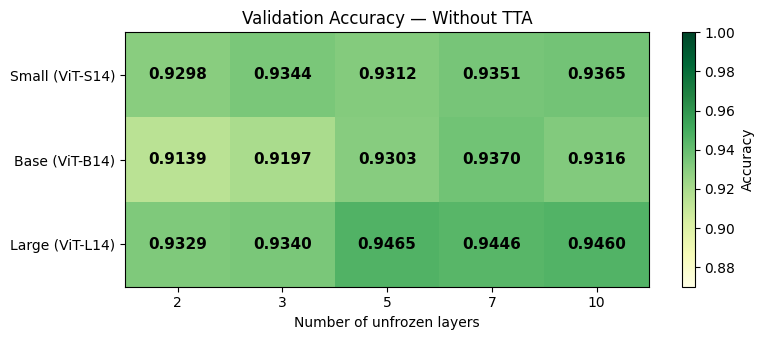
\includegraphics[width=\linewidth]{img/valacc_no_tta.png}
    \caption{Validation accuracy \textbf{without TTA}.}
    \label{fig:image1}
  \end{minipage}\hfill
  \begin{minipage}{0.45\textwidth}
    \centering
    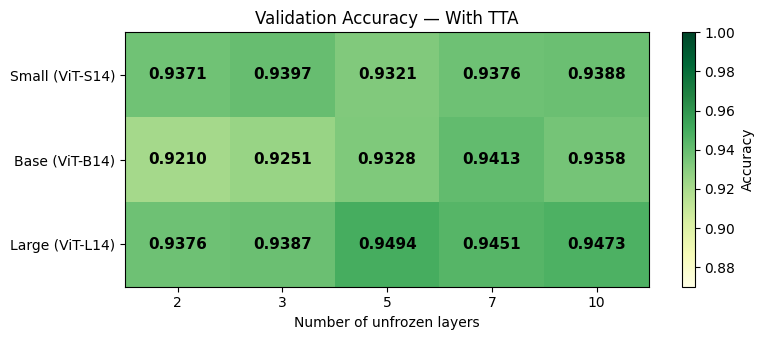
\includegraphics[width=\linewidth]{img/valacc_tta.png}
    \caption{Validation accuracy \textbf{with TTA}.}
    \label{fig:image2}
  \end{minipage}
\end{figure}

\paragraph{LOCO validation and Hibou-L exploration.}
Since the challenge targets generalization to unseen acquisition centers, we implemented a leave-one-center-out (LOCO) validation protocol over the training centers: $(3,4)\rightarrow0$, $(0,4)\rightarrow3$, and $(0,3)\rightarrow4$. This provides a less biased estimate of robustness to center-specific covariate shift than a random split. We also implemented an exploratory pipeline based on Hibou-L, a foundation model specifically designed for histopathology. This branch uses the model-specific preprocessing required by Hibou-L, including $224 \times 224$ inputs, Hibou normalization statistics, HED jittering, and a D4 geometric augmentation that samples exact rotations by multiples of $90^\circ$ and flip symmetries instead of arbitrary-angle rotations. The intended protocol was to compare several partial fine-tuning settings, in particular different numbers of unfrozen transformer blocks such as 2 versus 5, under the same LOCO scheme, then select the most stable configuration before final training on all centers. However, the Biomathematics-associated Ruche accounts were temporarily unavailable during their transfer to a new CDS laboratory, preventing us from completing the full Hibou-L LOCO benchmark in time for the report.

\paragraph{Hyperparameter optimization.}
Building on these observations, we performed a more in-depth hyperparameter optimization using Optuna. This search jointly explored architectural and optimization parameters, including learning rates for the head and backbone, number of unfrozen layers, augmentation strategies, and batch size. The best configuration obtained is summarized in Table~\ref{tab:best_config}. 

Interestingly, the optimal configuration does not rely on the additional domain generalization techniques such as MixStyle or StainMix, suggesting that the combination of partial fine-tuning, careful learning rate tuning, and TTA is sufficient to achieve strong generalization. The selected model (\texttt{dinov2\_vitl14} with 5 unfrozen layers) provides an effective balance between performance and computational cost, reaching a validation accuracy of $0.9559$, which constitutes our best result.

\section{Conclusion}

In this work, we tackled the problem of out-of-distribution generalization in histopathology image classification across acquisition centers. We proposed a pipeline combining a pretrained DINOv2 backbone with partial fine-tuning, stain-space data augmentation, and test-time augmentation. Through systematic experimentation and hyperparameter optimization, we identified a configuration that achieves strong performance on the validation set, demonstrating the effectiveness of our approach in mitigating domain shift. Future work could explore more advanced domain adaptation techniques, such as adversarial training or meta-learning, to further enhance robustness to unseen centers.


\clearpage  


\bibliography{bibliography}

\clearpage  

\appendix

\section{Details on the Data}

\begin{figure}[htbp]
\floatconts
  {fig:repartition}%
  {\caption{Distribution of samples across centers and classes.}}%
  {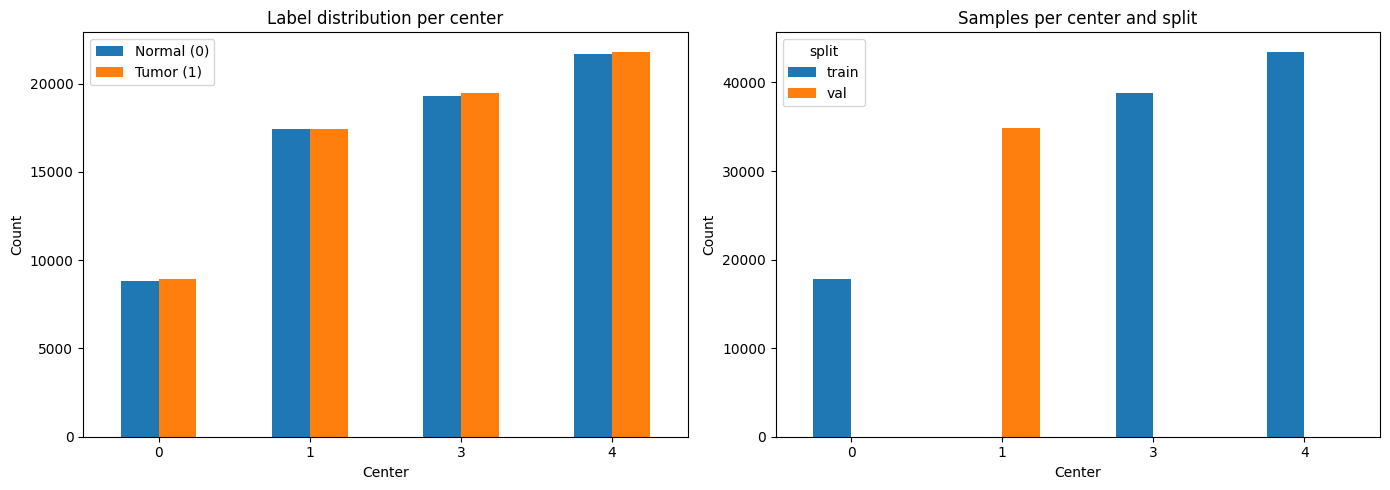
\includegraphics[width=\linewidth]{img/repartition.png}}
\end{figure}

\begin{figure}[htbp]
\floatconts
  {fig:umap}%
  {\caption{UMAP visualization of patch embeddings colored by \textbf{left:} training/validation split, and \textbf{right:} acquisition center.}}%
  {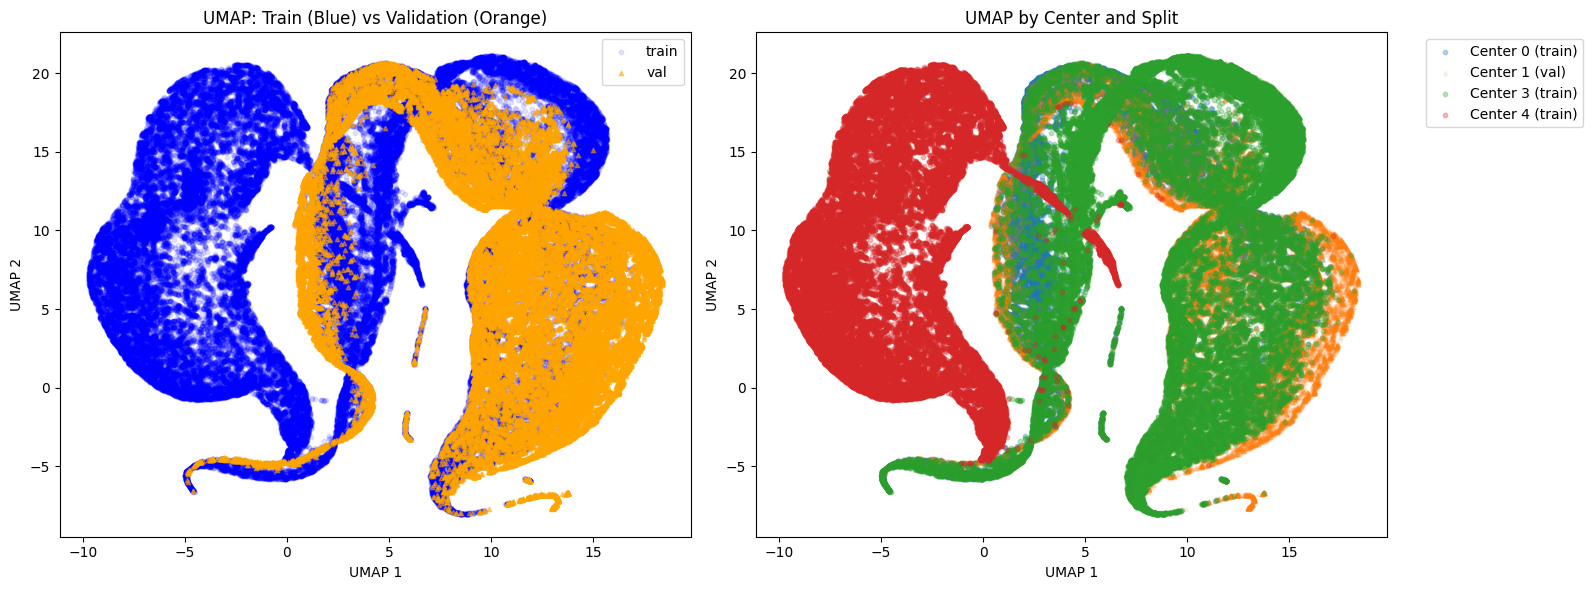
\includegraphics[width=\linewidth]{img/umap.png}}
\end{figure}

\section{Details on the Final Configuration}

\begin{table}[H]
\centering
\caption{Best configuration obtained after hyperparameter optimization.}
\label{tab:best_config}
\begin{tabular}{ll}
\bfseries Parameter & \bfseries Value \\
\hline
Model & \texttt{dinov2\_vitl14} \\
Number of unfrozen layers & 5 \\
Use MixStyle & False \\
MixStyle probability ($p$) & 0.5 \\
MixStyle alpha ($\alpha$) & 0.1 \\
Head learning rate & $1.36 \times 10^{-3}$ \\
Backbone learning rate & $6.25 \times 10^{-6}$ \\
Batch size & 32 \\
HED jittering strength ($\theta$) & 0.065 \\
Use StainMix & False \\
StainMix alpha & 0.3 \\
Stain bank size & 1000 \\
\end{tabular}
\end{table}

\end{document}
